\documentclass[conference]{IEEEtran}
\IEEEoverridecommandlockouts
\usepackage{cite}
\usepackage{amsmath,amssymb,amsfonts}
\usepackage{graphicx}
\usepackage{textcomp}
\usepackage{xcolor}
\usepackage{booktabs}
\usepackage{multirow}
\usepackage{url}
\def\BibTeX{{\rm B\kern-.05em{\sc i\kern-.025em b}\kern-.08em
    T\kern-.1667em\lower.7ex\hbox{E}\kern-.125emX}}

\makeatletter
\newcommand{\linebreakand}{%
  \end{@IEEEauthorhalign}
  \hfill\mbox{}\par
  \mbox{}\hfill\begin{@IEEEauthorhalign}
}
\makeatother

\begin{document}

\title{AIRE-Trace: A Standardized Prospective Evaluation and Trajectory Risk Decomposition Framework for Online Agent-Failure Warning}

\author{\IEEEauthorblockN{B.~Naveen~Raj}
\IEEEauthorblockA{\textit{Dept.\ of CSE (AIML)} \\
\textit{K.S. Rangasamy College of Technology}\\
Tiruchengode--637215, India \\
naveenrajbv1@gmail.com}
\and
\IEEEauthorblockN{C.~Janani}
\IEEEauthorblockA{\textit{Assistant Professor}\\
\textit{Dept.\ of CSE (AIML)} \\
\textit{K.S. Rangasamy College of Technology}\\
Tiruchengode--637215, India \\
srijanani2030@gmail.com}
\linebreakand
\IEEEauthorblockN{P.~Krishnamoorthi}
\IEEEauthorblockA{\textit{Dept.\ of CSE (AIML)} \\
\textit{K.S. Rangasamy College of Technology}\\
Tiruchengode--637215, India \\
pkrishnamoorthi126@gmail.com}
\and
\IEEEauthorblockN{L.~Maadhava Kumar}
\IEEEauthorblockA{\textit{Associate Software Developer} \\
\textit{Mphasis}\\
Chennai, India \\
maadhava05@gmail.com}
}

\maketitle

\begin{abstract}
The increasing deployment of autonomous tool-using AI agents creates
demand for mechanisms that provide prospective warning of task failure
from partial execution trajectories, rather than retrospective diagnosis
after failure has occurred. Prior work on online agent-failure warning
has demonstrated that prefix-based failure prediction is viable, but
existing methods each use their own datasets, prefix definitions,
calibration procedures, and metrics, making comparative claims difficult
to interpret.

This paper presents AIRE-Trace, a standardized prospective evaluation
protocol for online agent-failure warning that fixes information
visibility, failure-target definition, alert semantics, calibration
procedure, false-alarm constraints, and lead-time measurement. We
further propose trajectory risk decomposition (\texttt{dyn\_comp}), which
combines static and dynamic risk signals from trajectory prefixes to
improve prospective recall under the protocol's false-alarm budget.

The protocol is applied to representative heuristic (H1--H4), classical
machine-learning (M1), sequence-model (S1, S2), and risk-decomposition
(\texttt{dyn\_comp}) warning methods on 636 reconstructed episodes
(a 19.18\% strict-retention sample of the 3{,}316 declared source rows),
split task-disjointly into TRAIN~(163),
CALIBRATION~(57), and TEST~(416). Under the stringent 5\% false-alarm
rate (FAR) constraint, \texttt{dyn\_comp} achieved a modest prospective
Recall@FAR of 0.1167
(FAR~=~0.0404), compared with the M1 baseline at 0.0078
(FAR~=~0.0303). A paired episode-cluster bootstrap ($B$~=~10{,}000)
confirmed the difference ($\Delta$~=~+0.1089, 95\%~CI
[0.0706,~0.1496], $p_{\mathrm{adj}}$~=~$9.999 \times 10^{-5}$).
Baseline AUROC ranged from 0.5074 to 0.6371. Feature ablation
showed that omitting cumulative error and retry signals yielded the
largest observed drop in discrimination ($\Delta$AUROC~=~$-$0.1069).
Pairwise Direction
Consistency across seven baselines was 0.8294 (21/21 informative pairs),
indicating largely but not universally consistent rankings.
\end{abstract}

\begin{IEEEkeywords}
Agentic systems, failure warning, prospective evaluation, trajectory
analysis, standardized benchmarking, online monitoring, calibration,
bootstrap inference, risk decomposition.
\end{IEEEkeywords}

%% ====================================================================
%%  I. INTRODUCTION
%% ====================================================================
\section{Introduction}

The deployment of autonomous agentic systems---agents that plan, invoke
tools, and execute multi-step tasks with limited human oversight---has
raised reliability questions that standard outcome benchmarking cannot
fully answer. Benchmarks such as AgentBench~\cite{b1},
AgentBoard~\cite{b2}, and GAIA~\cite{b3} measure whether an agent
ultimately succeeds or fails, but this final-outcome evaluation is
insufficient for monitoring purposes: by the time the outcome is
observed, the agent has already consumed resources and potentially caused
unrecoverable side effects.

\textit{Prospective failure warning} addresses a complementary question:
given only the portion of the trajectory observed so far (a prefix), can
a monitor produce a timely alert that the episode will likely fail
\textit{before} the outcome is known? This early-warning capability
would enable intervention---pausing the agent, escalating to human
review, or switching strategies---before failure becomes irreversible.

Recent work has shown that prefix-based failure prediction is
achievable. PrefixGuard~\cite{b7} demonstrates prefix-based warning
monitors on WebArena and TerminalBench. AgentForesight~\cite{b8} employs
an RL-trained 7B-parameter auditor. Trajectory Guard~\cite{b9} applies
real-time sequence anomaly detection. However, these methods each use
their own datasets, prefix definitions, calibration procedures, and
metrics. No existing work cross-compares heuristic, classical-ML, and
sequence-model warning methods under one fixed protocol, making it
unclear whether reported advantages are robust to a common evaluation
protocol or partially artifacts of differing evaluation conditions.

AIRE-Trace addresses this gap with two contributions:
\begin{enumerate}
\item A \textbf{standardized prospective evaluation protocol} for online
      agent-failure warning---fixing information visibility (pre-onset
      prefix only), failure-target definition, alert semantics,
      calibration procedure (FAR~$\leq$~5\%), and statistical inference
      (episode-cluster bootstrap with Holm--Bonferroni correction).
\item \textbf{Trajectory risk decomposition} (\texttt{dyn\_comp}), which
      combines static base-rate and dynamic trajectory-prefix risk
      signals to improve prospective recall under the protocol's
      false-alarm constraint.
\end{enumerate}

AIRE-Trace is an \textit{offline evaluator} of pre-recorded agent
trajectories. It does not perform live intervention.

\textbf{Research Question.} \textit{Do comparative performance claims
for online agent-failure warning methods remain consistent when methods
are evaluated under identical information, target, alert, calibration,
lead-time, and compute constraints?}

%% ====================================================================
%%  II. RELATED WORK AND COMPARATIVE GAP
%% ====================================================================
\section{Related Work and Comparative Gap}

\subsection{Agent Outcome Benchmarking}
Outcome benchmarks~\cite{b1,b2,b3} establish performance baselines for
agent capabilities but do not provide mechanisms for prospective
mid-execution monitoring. TRAIL~\cite{b4} articulates the need for
robust evaluation of agentic traces, presenting 148 human-annotated
traces for trace-debugging evaluation.

\subsection{Retrospective Failure Attribution}
Post-hoc attribution methods identify where or why a trajectory went
wrong after failure has occurred. AgentRx~\cite{b5} provides post-hoc
localization of critical failure steps. Who\&When Pro~\cite{b6}
addresses retrospective attribution using 12{,}326 trajectories.
AgentProcessBench~\cite{b11} introduces step-level quality evaluation
with 8{,}509 human-labeled annotations. These approaches require the
complete trajectory and are retrospective by construction.

\subsection{Prospective Agent-Failure Warning}
PrefixGuard~\cite{b7} achieves AUPRC of 0.900 on WebArena and 0.557 on
TerminalBench under its own evaluation protocol. Direct numerical
comparison with AIRE-Trace results is not appropriate due to differences
in prefix representation, feature regime, and calibration protocol.
AgentForesight~\cite{b8} employs an RL-trained auditor. Trajectory
Guard~\cite{b9} applies sequence anomaly detection. Advani~\cite{b10}
characterizes false success in LLM agents, showing that TF-IDF detectors
achieve AUROC 0.83--0.95 for false-success detection. These works
collectively establish prospective warning as a viable research direction
but operate in isolation without cross-comparison under a common
protocol.

\subsection{Evaluation Methodology}
Cameron, Gelbach, and Miller~\cite{b12} establish the pairs cluster
bootstrap as the appropriate inference procedure when observations are
dependent within clusters. Holm~\cite{b13} introduced the sequentially
rejective multiple test procedure for familywise error rate control.

%% ====================================================================
%%  III. AIRE-TRACE METHODOLOGY
%% ====================================================================
\section{AIRE-Trace Methodology}

The AIRE-Trace prospective evaluation protocol enforces strict separation
between pre-onset trajectory monitoring, offline threshold calibration,
and test-set prospective evaluation, as illustrated in
Fig.~\ref{fig:arch}.

\begin{figure}[t]
\centering
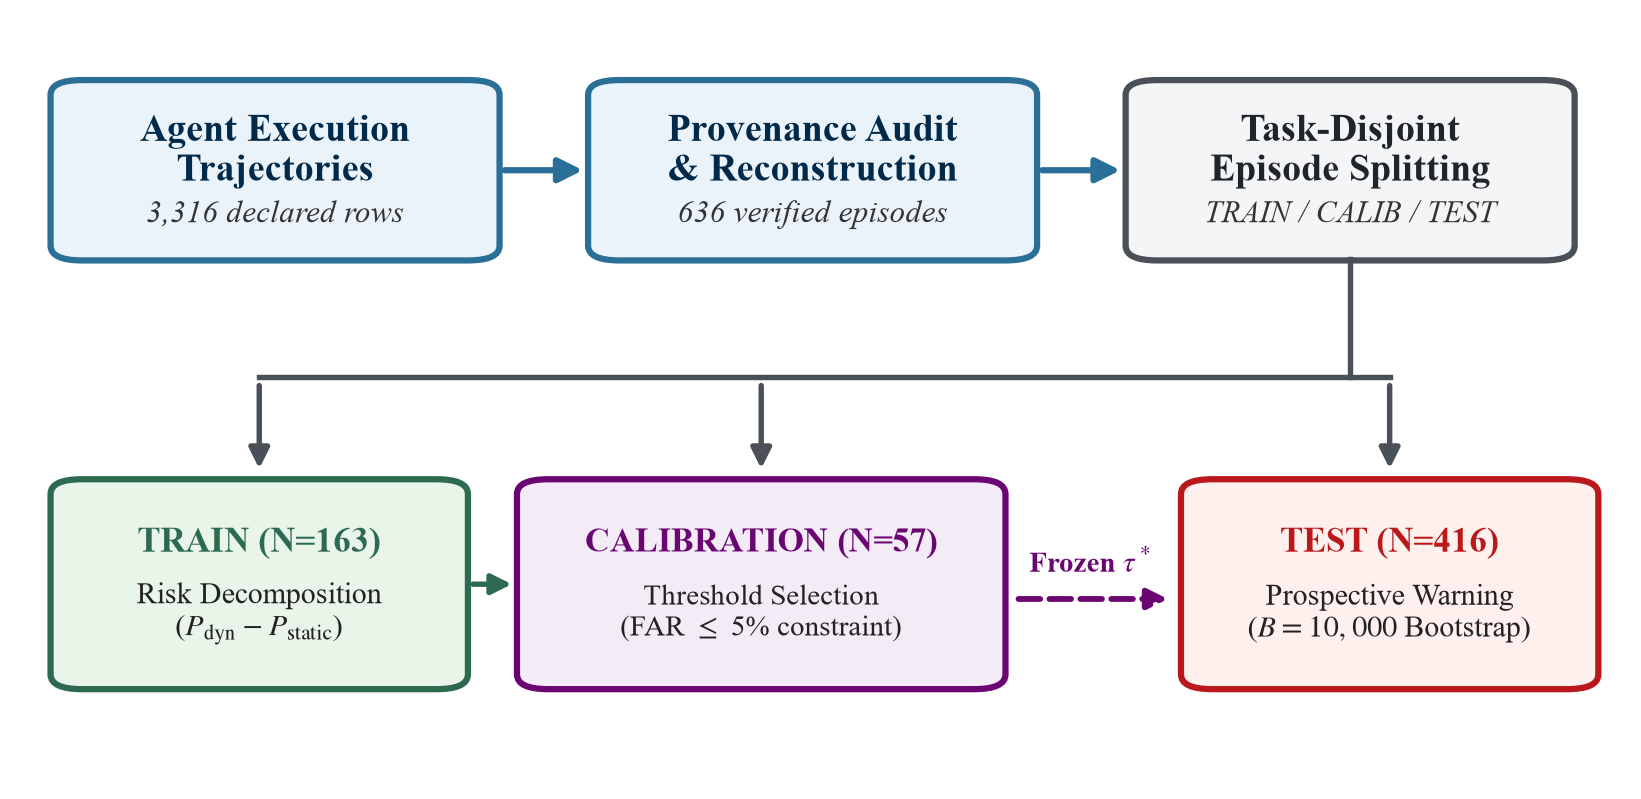
\includegraphics[width=\columnwidth]{figures/fig1_aire_trace_architecture.png}
\caption{AIRE-Trace standardized prospective evaluation pipeline.
Trajectories are provenance-audited before episode-level splitting;
trainable methods are fitted on TRAIN, operating thresholds are selected
on CALIBRATION under the FAR constraint, and frozen thresholds are
applied to the TEST population.}
\label{fig:arch}
\end{figure}

\subsection{Prospective Evaluation Protocol}

An agent episode consists of a sequence of events
$e_1, e_2, \ldots, e_T$ produced by an autonomous agent executing a
task. Each event contains role information (agent, tool, user, system),
action type, tool names, and error indicators. The episode has an
eventual outcome: \texttt{eventual\_success} or
\texttt{eventual\_failure}.

For TerminalBench episodes, the failure onset is defined as
$t_{\mathrm{onset}} = \min(\texttt{incorrect\_step\_ids})$. Episodes
lacking this annotation are excluded from onset-dependent metrics
(Recall@FAR, lead time) but remain eligible for ranking metrics (AUROC,
AUPRC).

At checkpoint $t \in \{1, \ldots, \min(T_i, K)\}$ with horizon $K=30$,
a monitor accesses only the prefix $(e_1, \ldots, e_t)$. The checkpoint
schedule is outcome-independent and episode-symmetric. An alert at
checkpoint $t$ is \textit{prospective} if and only if
$t \leq t_{\mathrm{onset}}$; an alert at $t > t_{\mathrm{onset}}$ is a
\textit{late detection} and is reported separately in the operational
analysis. The prospective evaluation semantics are illustrated in
Fig.~\ref{fig:prefix}.

\begin{figure}[t]
\centering
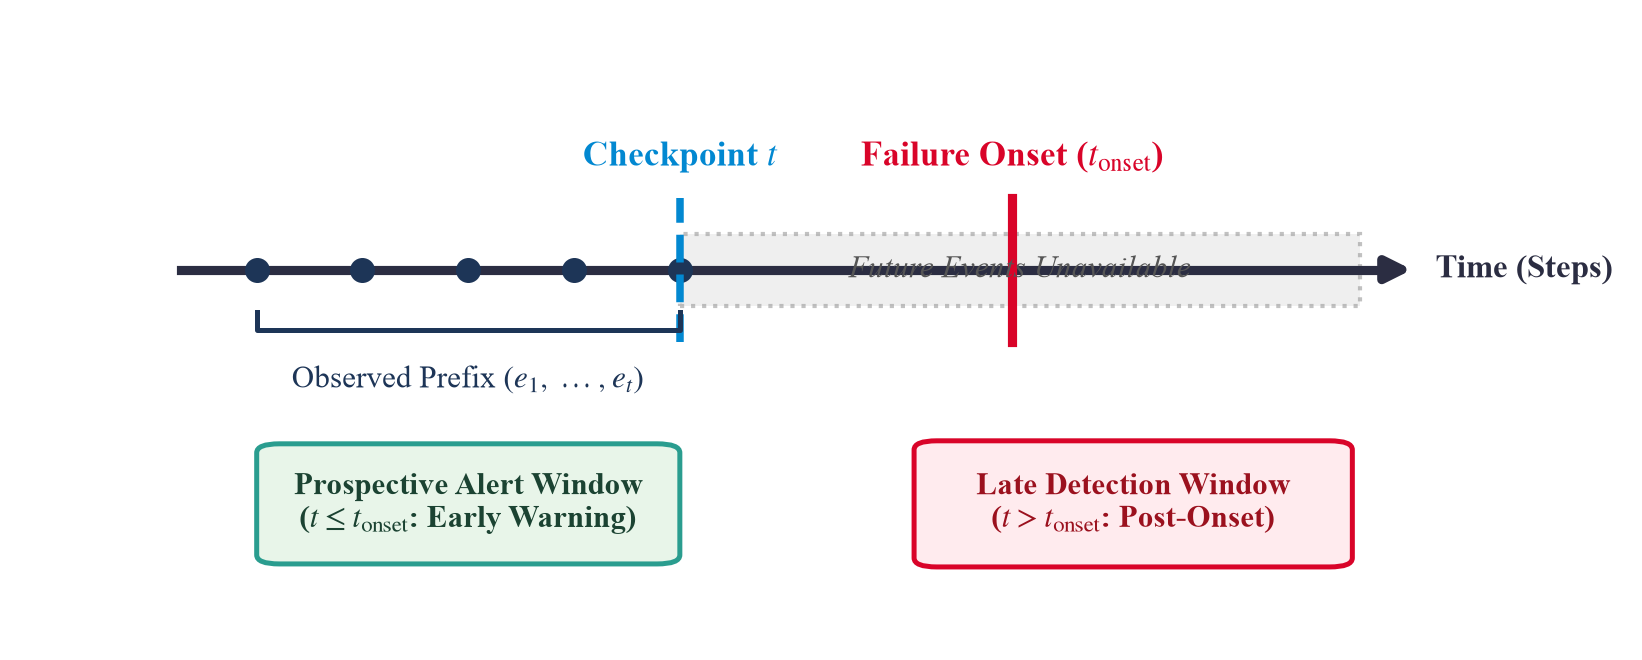
\includegraphics[width=\columnwidth]{figures/fig3_prospective_prefix.png}
\caption{Prospective prefix evaluation semantics. At each checkpoint,
the monitor observes only the trajectory prefix. Alerts at or before the
annotated failure onset constitute prospective detections; alerts after
onset are analyzed separately as late detections.}
\label{fig:prefix}
\end{figure}

Given a prefix at checkpoint $t$, a monitor produces a risk score
$s(e_1,\ldots,e_t) \in [0,1]$. An alert is raised when
$s \geq \tau$ for a calibrated threshold $\tau$. Episode-level FAR is defined in~\eqref{eq:far}:
\begin{equation}
\mathrm{FAR} = \frac{|\{i : \mathrm{success}(i) \wedge \exists\, t:\,\mathrm{alert}_t\}|}{|\{i : \mathrm{success}(i)\}|}
\label{eq:far}
\end{equation}

Each episode contributes equally to prefix-level metric computation via
episode-balanced weighting: $w_{i,t} = 1 / \min(T_i, K)$.

\textbf{Evaluation Modes.}
\textit{Mode~A} (TerminalBench, primary): supports AUROC, AUPRC, Brier,
ECE, prospective Recall@FAR, lead time, and late-detection analysis.
\textit{Mode~B} ($\tau^2$-Bench, diagnostic): reports
eventual-outcome ranking metrics only. Mode~B metrics must not be
compared directly to Mode~A metrics.

\subsection{Dataset and Task-Disjoint Splits}

The primary corpus is Tracebench (3{,}316 declared source rows). After
provenance auditing and reconstruction, 2{,}655 rows were structurally
invalid due to missing trajectory artifacts, 25 contained unreachable
artifact paths, and network recovery attempts yielded zero additional
valid episodes, leaving 636 canonical episodes (19.18\%) for
benchmarking. These exclusions represent strict structural
data-availability attrition; however, missingness cannot be assumed
to be missing completely at random (MCAR). Consequently, systematic
selection bias cannot be ruled out, and all empirical findings remain
formally bounded to this audited 636-episode cohort. The overall
pipeline structure is depicted in Fig.~\ref{fig:arch}.

The 636 episodes are split task-disjointly (entire episode to exactly
one split): TRAIN (163), CALIBRATION (57), TEST (416). The TEST
population contains 317 failed episodes (257 with valid onset
annotations, 60~without), and 99 successful episodes.

\subsection{Threshold Calibration and Alert Semantics}

The calibration procedure selects
$\tau^* = \arg\max_\tau \mathrm{Recall}(\tau)$ subject to
$\mathrm{FAR}_{\mathrm{calib}}(\tau) \leq 0.05$, on the CALIBRATION
split only. Ties are broken by lower FAR first, then higher threshold.
The selected threshold $\tau^*$ is frozen before TEST evaluation.

\subsection{Trajectory Risk Decomposition}

The trajectory risk decomposition method (\texttt{dyn\_comp}) decomposes
the failure risk score into an empirical static task-difficulty prior
and a dynamic prefix-derived risk signal in~\eqref{eq:dyn_comp}:
\begin{equation}
s_{\mathrm{dyn\_comp}}(t) = P_{\mathrm{M1}}(\mathrm{fail} \mid e_{1:t}) - P_{\mathrm{static}}(\mathrm{fail} \mid \mathrm{task})
\label{eq:dyn_comp}
\end{equation}
where $P_{\mathrm{M1}}(\mathrm{fail} \mid e_{1:t})$ is the dynamic
failure probability predicted by the logistic baseline M1 from the 13
prefix features $\mathbf{x}_{1:t}$, and
$P_{\mathrm{static}}(\mathrm{fail} \mid \mathrm{task})$ is a static prior
fitted on the TRAIN split from task category and difficulty failure base
rates. Both components are strictly computable at prefix checkpoint $t$
without future trajectory leakage. The residual score
$s_{\mathrm{dyn\_comp}}(t) \in [-1, 1]$ isolates excess dynamic risk
relative to static task expectations. The operating threshold
$\tau^* = 0.5522$ is calibrated on CALIBRATION under the
$\mathrm{FAR} \leq 5\%$ constraint, identical to all baselines.

%% ====================================================================
%%  IV. EXPERIMENTAL SETUP
%% ====================================================================
\section{Experimental Setup}

\subsection{Models and Baselines}

Seven baseline methods and one proposed method are registered (Table~\ref{tab:models}):

\begin{table}[t]
\centering
\caption{Warning Method Registry}
\label{tab:models}
\begin{tabular}{@{}llp{3.7cm}@{}}
\toprule
ID & Family & Method / Key Parameters \\
\midrule
H1 & Heuristic & Tool-error rate (min-max norm) \\
H2 & Heuristic & Retry-count (min-max norm) \\
H3 & Heuristic & Repeated-action (min-max norm) \\
H4 & Heuristic & Combined (sigmoid z-score avg) \\
M1 & Classical & Logistic Regression (C=1.0, lbfgs) \\
S1 & Sequence$^\dagger$ & Random Forest (100 trees, depth=6) \\
S2 & Sequence & GRU (hidden=64, 1 layer, 10 epochs) \\
\texttt{dyn\_comp} & Proposed & Trajectory risk decomposition \\
L  & Semantic & LLM monitor (\textit{not evaluated}) \\
\bottomrule
\multicolumn{3}{@{}l}{\footnotesize $^\dagger$S1 classified Sequence by registry; implemented as}\\
\multicolumn{3}{@{}l}{\footnotesize Random Forest tabular ensemble. L skipped: RTX~2050, 4\,GB.}
\end{tabular}
\end{table}

All trainable models use 13 Category-A structural features computed from
the prefix: \texttt{feat\_steps\_so\_far} (cumulative step count),
four actor-role counts (agent, tool, user, system), three action-type
counts (message, tool\_call, tool\_result),
\texttt{feat\_tool\_error\_count} (cumulative tool errors),
\texttt{feat\_retry\_count} (consecutive error sequences),
\texttt{feat\_unique\_tools\_used}, \texttt{feat\_tool\_call\_ratio},
and \texttt{feat\_repeated\_action\_last2}. Models are fitted on TRAIN
with episode-balanced sample weights; all use random seed~42.
S1 is registered within the sequence-comparison tier as a non-recurrent
competitive baseline that maps cumulative prefix trajectory statistics
into a tabular ensemble, directly contrasting with S2's hidden-state GRU
recurrence.

\subsection{Metrics and Statistical Analysis}

\textbf{Ranking metrics} (prefix-level, episode-balanced): AUROC, AUPRC,
Brier Score, ECE.

\textbf{Operational metrics} (episode-level): FAR (denominator: 99
successful TEST episodes), Recall@FAR (denominator: 257 valid annotated
failure episodes).

\textbf{Bootstrap inference:} Paired episode-cluster bootstrap. Standard
baseline comparisons use $B$~=~1{,}000 iterations. The primary
\texttt{dyn\_comp} vs.\ M1 comparison uses $B$~=~10{,}000 iterations.
Episodes are resampled with replacement at the episode level (not prefix
level) to preserve within-episode dependence~\cite{b12}. Frozen
thresholds are held constant across resamples. Prefix-level resampling
is incorrect because prefixes within the same episode share the outcome
label, violating independence and producing artificially narrow CIs.

\textbf{Multiple-comparison correction:} Holm--Bonferroni step-down
correction~\cite{b13} across predefined comparison families,
$\alpha$~=~0.05.

\textbf{Pairwise Direction Consistency (PDC):} For each model pair
$(A,B)$, wins $W$ and losses $L$ are counted across AUROC, AUPRC,
Recall@FAR, and ECE. Pairs with $W$+$L$=0 are excluded. If $W$=2 and
$L$=2, pair PDC~=~0.50; otherwise PDC~=~$\max(W,L)/(W+L)$. Overall PDC
is the arithmetic mean of informative pair PDCs, always reported with
its coverage figure.

%% ====================================================================
%%  V. RESULTS
%% ====================================================================
\section{Results}

\subsection{Primary Prospective Warning Results}

Table~\ref{tab:primary} presents the primary Mode~A TEST performance.
Under the FAR~$\leq$~5\% constraint, \texttt{dyn\_comp} achieved
Recall@FAR of 0.1167 with FAR of 0.0404 (frozen threshold 0.5522).
The M1 baseline achieved Recall@FAR of 0.0078 with FAR of
0.0303 (frozen threshold 0.98). All remaining baselines achieved
Recall@FAR of 0.0000, with the exception of H3, whose Recall@FAR is
undefined because its calibration FAR reached 1.000 (the 5\% constraint
was not achievable).

\begin{table}[t]
\centering
\caption{Primary Mode~A TEST Performance ($K$=30, FAR~$\leq$~5\%)}
\label{tab:primary}
\begin{tabular}{@{}lcccc@{}}
\toprule
Model & $\tau$ & AUROC & Recall@FAR & FAR \\
\midrule
H1 & 0.86 & 0.6205 & 0.0000 & 0.0000 \\
H2 & 0.89 & 0.5752 & 0.0000 & 0.0000 \\
H3 & 0.01 & 0.5074 & undef.$^\dagger$ & 1.0000 \\
H4 & 0.93 & 0.6135 & 0.0000 & 0.0202 \\
M1 & 0.98 & 0.6215 & 0.0078 & 0.0303 \\
S1 & 0.97 & 0.6371 & 0.0000 & 0.0404 \\
S2 & 0.74 & 0.5496 & 0.0000 & 0.0000 \\
\texttt{dyn\_comp} & 0.5522 & 0.3593 & \textbf{0.1167} & 0.0404 \\
\bottomrule
\multicolumn{5}{@{}l}{\footnotesize $^\dagger$H3 Recall@FAR undefined:
calibration FAR = 1.000.}
\end{tabular}
\end{table}

In Table~\ref{tab:primary}, \texttt{dyn\_comp}'s protocol-consistent
episode-balanced prefix AUROC is 0.3593. Because \texttt{dyn\_comp}
subtracts the static task-difficulty prior ($P_{\mathrm{static}}$, whose
observed failure-ranking AUROC is 0.6940), early non-erroneous prefixes
of difficult failed episodes can yield negative residual scores, producing
a sub-0.5 global prefix AUROC. The residual is an operational anomaly
detector rather than a monotonic global risk score; the primary
evaluation remains thresholded prospective warning. At the frozen
operating threshold ($\tau^* = 0.5522$), \texttt{dyn\_comp} fires only on
extreme positive dynamic risk spikes, achieving Recall@FAR of 0.1167 at
FAR of 0.0404, while the M1 baseline yields Recall@FAR of 0.0078 at FAR
of 0.0303.

\textbf{Primary paired comparison.} Table~\ref{tab:bootstrap} presents
the primary \texttt{dyn\_comp} vs.\ M1 bootstrap result.

\begin{table}[t]
\centering
\caption{Primary \texttt{dyn\_comp} vs.\ M1 Bootstrap Comparison}
\label{tab:bootstrap}
\begin{tabular}{@{}ll@{}}
\toprule
Quantity & Value \\
\midrule
Metric & Recall@FAR (prospective) \\
Observed $\Delta$ (dyn\_comp $-$ M1) & +0.1089 \\
95\% CI & [0.0706, 0.1496] \\
Bootstrap $B$ & 10{,}000 \\
Bootstrap unit & Episode-cluster (joint) \\
$p_{\mathrm{adj}}$ & $9.999 \times 10^{-5}$ \\
Reject $H_0$ at $\alpha=0.05$ & Yes \\
\texttt{dyn\_comp} FAR & 0.0404 \\
M1 FAR & 0.0303 \\
\bottomrule
\end{tabular}
\end{table}

\subsection{Baseline Comparative Results}

Among the seven baselines, Mode~A AUROC ranged from 0.5074 (H3) to
0.6371 (S1). S1 (Random Forest, AUROC = 0.6371, 95\%~CI
[0.5885,~0.6745]) achieved the highest observed AUROC, as visualized
in Fig.~\ref{fig:auroc}.

\begin{figure}[t]
\centering
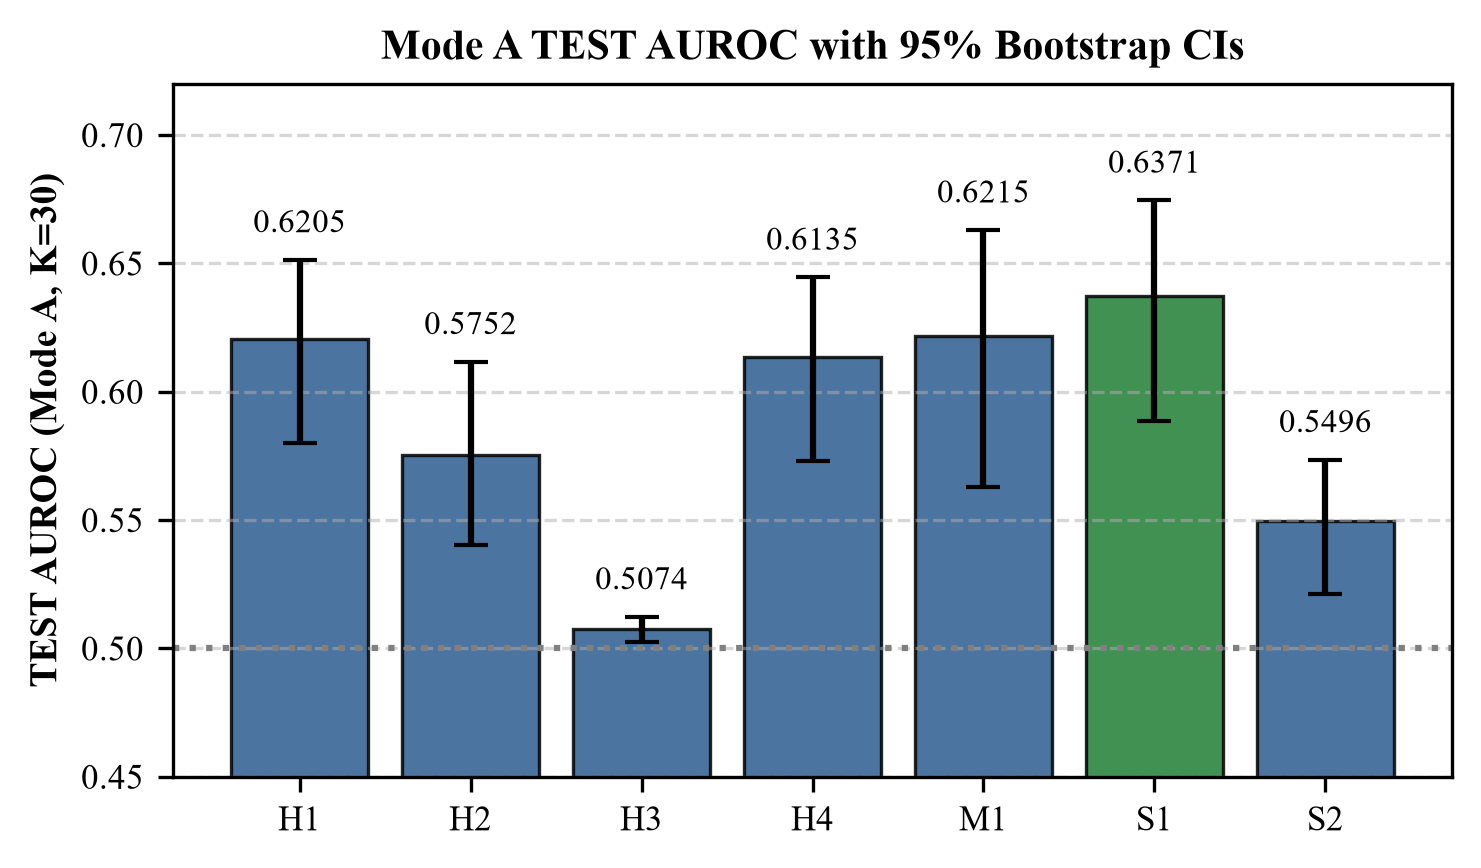
\includegraphics[width=\columnwidth]{figures/fig4_mode_a_auroc.png}
\caption{Mode~A TEST AUROC for baseline warning methods ($K$=30). Error
bars denote 95\% episode-cluster bootstrap confidence intervals. S1
(Random Forest) achieved the highest observed AUROC (0.6371).}
\label{fig:auroc}
\end{figure}

Paired episode-cluster bootstrap testing ($B$~=~1{,}000,
Holm--Bonferroni correction) showed S1 had statistically significant
AUROC advantages over S2 ($\Delta$~=~+0.0875, $p_{\mathrm{adj}}$~=~0.006),
H2 ($\Delta$~=~+0.0619, $p_{\mathrm{adj}}$~=~0.006),
and H3 ($\Delta$~=~+0.1297, $p_{\mathrm{adj}}$~=~0.006),
but not over M1, H1, or H4. For AUPRC, S1's advantage was statistically
significant only against S2 ($p_{\mathrm{adj}}$~=~0.012).

Despite S1's highest AUROC, its prospective Recall@FAR at FAR~$\leq$~5\%
was 0.0000, illustrating a fundamental gap between discriminative
performance and operational early-warning utility.

\textbf{FAR sensitivity.} S1 evaluated at FAR targets of 1\%, 5\%, and
10\% achieved identical frozen thresholds at 1\% and 5\% ($\tau$~=~0.97,
Recall@FAR~=~0.0000). At 10\% FAR target ($\tau$~=~0.93),
Recall@FAR improved to 0.0973, indicating the recall/FAR trade-off.

\subsection{Ranking Consistency}

The overall Pairwise Direction Consistency (PDC) across the seven
baselines (H1, H2, H3, H4, M1, S1, S2) was \textbf{0.8294} with
coverage of 0.881 across 21/21 informative pairs. This indicates that
the majority of pairwise ranking directions are consistent across
metrics, while approximately 17\% of comparisons contain at least one
metric disagreement. \texttt{dyn\_comp} is not included in this baseline
PDC matrix.

\subsection{Ablation and Robustness}

Feature ablation (A0--A6) on S1 under the frozen protocol is summarized
in Table~\ref{tab:ablation}. Removing error and retry signals
(\texttt{feat\_tool\_error\_count} and \texttt{feat\_retry\_count};
ablation A4) produced the largest observed discrimination degradation
($\Delta$AUROC~=~$-$0.1069, from 0.6371 to 0.5302). All other
ablations produced $|\Delta\mathrm{AUROC}| < 0.004$. This identifies
error and retry signals as the feature group whose removal produced
the largest observed discrimination loss under S1 and the evaluated
feature set.

\begin{table}[t]
\centering
\caption{S1 Feature Ablation Results (Mode~A, $K$=30)}
\label{tab:ablation}
\begin{tabular}{@{}llcc@{}}
\toprule
ID & Removed Features & AUROC & $\Delta$ \\
\midrule
A0 & None (full baseline) & 0.6371 & --- \\
A1 & \texttt{steps\_so\_far} & 0.6357 & $-$0.0014 \\
A2 & 4 actor-role features & 0.6335 & $-$0.0036 \\
A3 & 3 action-type features & 0.6383 & +0.0012 \\
A4 & \texttt{error\_count + retry} & \textbf{0.5302} & $-$\textbf{0.1069} \\
A5 & \texttt{tools + ratio} & 0.6360 & $-$0.0011 \\
A6 & \texttt{repeated\_action} & 0.6341 & $-$0.0030 \\
\bottomrule
\end{tabular}
\end{table}

\subsection{Operational Analysis}

The operational analysis examines false alarms, late detections, and
alert burden under frozen thresholds, summarized in
Table~\ref{tab:operational}. H3 (FAR~=~1.000) alerts on all
99 successful TEST episodes and 19.84\% of valid failure episodes
received only late (post-onset) alerts (accounting for 3{,}339 late
alerts out of 8{,}012 total alerts across the TEST split). This
illustrates why the onset boundary must be explicitly enforced:
H3's activity represents retrospective diagnosis, not prospective
warning.

\begin{table}[t]
\centering
\caption{Operational Warning Profile (Mode~A, $K$=30, Frozen $\tau$)}
\label{tab:operational}
\begin{tabular}{@{}lccccc@{}}
\toprule
Model & \shortstack{FA\\Ep.} & \shortstack{TEST\\FAR} & \shortstack{Only-Late\\Ep. (\%)} & \shortstack{Total\\Alerts} & \shortstack{Mean/\\Ep.} \\
\midrule
H1 & 0 & 0.0000 & 2 (0.78\%) & 19 & 0.046 \\
H2 & 0 & 0.0000 & 2 (0.78\%) & 16 & 0.039 \\
H3 & 99 & 1.0000 & 51 (19.84\%) & 8{,}012 & 19.260 \\
H4 & 2 & 0.0202 & 8 (3.11\%) & 119 & 0.286 \\
M1 & 3 & 0.0303 & 10 (3.89\%) & 161 & 0.387 \\
S1 & 4 & 0.0404 & 16 (6.23\%) & 25 & 0.060 \\
S2 & 0 & 0.0000 & 10 (3.89\%) & 107 & 0.257 \\
\bottomrule
\multicolumn{6}{@{}l}{\footnotesize FA Ep.: false-alarm episodes (out of 99 successful TEST episodes).}\\
\multicolumn{6}{@{}l}{\footnotesize Only-Late: failure episodes with solely post-onset alerts (out of 257).}
\end{tabular}
\end{table}

Among models operating within the FAR target, S1 produced the lowest
alert burden (25 total alerts, max 2 per episode) but zero prospective
recall. \texttt{dyn\_comp}, with 0.0404 FAR, achieved the only non-trivial
prospective recall (0.1167) among all evaluated methods.

%% ====================================================================
%%  VI. DISCUSSION AND LIMITATIONS
%% ====================================================================
\section{Discussion and Limitations}

\subsection{The Operational Recall Collapse}

The most critical finding is the collapse of prospective Recall@FAR
under the 5\% FAR constraint: the baselines with a defined Recall@FAR
achieved zero or near-zero prospective recall; H3 was undefined because
the 5\% FAR constraint was not achievable. S1's AUROC of 0.6371
demonstrates meaningful probabilistic discrimination, but the
discriminative signal is insufficient to generate threshold-based
alerts on individual failure episodes before onset without FAR
violations. \texttt{dyn\_comp}'s Recall@FAR of 0.1167
represents a statistically significant improvement over M1's 0.0078, but
the absolute recall remains modest. The gap between discriminative
ranking capability and operational early-warning utility is a structural
finding of this evaluation.

\subsection{Selective Statistical Significance}

The bootstrap-tested AUROC advantages for S1 are statistically
significant only against S2, H2, and H3.
Its advantages over M1, H1, and H4 are not statistically significant
after Holm--Bonferroni correction. The empirical ordering
S1~$>$~M1~$>$~H1~$>$~H4 by point estimate does not reflect universally
distinguishable statistical differences.

\subsection{Limitations}

\textbf{Population coverage and selection bias.} The 636 retained
episodes represent 19.18\% of the 3{,}316 declared source rows. Because
exclusion was driven by artifact corruption and unreachable paths
rather than random subsampling, the retained cohort may systematically
differ from the excluded episodes across task complexity, agent run
length, or failure distribution. The reported failure distributions and
warning behaviors are valid within the audited canonical population,
but generalization to the uncurated source population remains
unverified.

\textbf{Incomplete onset annotation.} 60 of 317 TEST failure episodes
(18.9\%) lack onset annotations. These episodes are excluded from
onset-dependent Recall@FAR and late-detection analysis but remain
available for ranking metrics. Systematic differences between annotated
and unannotated episodes may affect reported prospective-warning rates.

\textbf{LLM-monitor evaluation.} The L~(LLM-monitor) model was not
evaluated because the available hardware (RTX~2050, 4\,GB VRAM) could
not support protocol-compliant evaluation over the full dataset. No
conclusions about L's prospective performance can be drawn.

\textbf{Domain scope.} Transferability of the protocol and results is
restricted to the evaluated tool-use coding-task domain. Generalization
to other agent types or task domains has not been established.

\textbf{Offline evaluation.} AIRE-Trace is an offline evaluator of
recorded trajectories, not a runtime intervention mechanism. Deployment
considerations are outside the scope of this work.

%% ====================================================================
%%  VII. CONCLUSION
%% ====================================================================
\section{Conclusion}

This study evaluated prospective failure warning from trajectory-prefix
information under an explicit separation between pre-onset prediction
and post-onset alerting, using 636 reconstructed episodes with a
task-disjoint TRAIN/CALIBRATION/TEST split and frozen calibration
thresholds.

Across seven baselines at $K$=30, Mode~A AUROC ranged from 0.5074 to
0.6371. Under the 5\% FAR constraint, the baselines with a defined
Recall@FAR achieved zero or near-zero prospective recall (H3 was
undefined because its calibration FAR reached 1.000). Trajectory
risk decomposition (\texttt{dyn\_comp}) achieved Recall@FAR of 0.1167,
a statistically significant improvement over M1
($\Delta$~=~+0.1089, 95\%~CI [0.0706,~0.1496],
$p_{\mathrm{adj}}$~=~$9.999 \times 10^{-5}$, $B$~=~10{,}000
episode-cluster bootstrap).

Feature ablation confirmed that omitting error and retry signals
produced the largest observed discrimination loss ($\Delta$AUROC = $-$0.1069
at A4). PDC of
0.8294 across 21 informative baseline pairs indicates largely consistent
but not universal ranking stability. The evaluated trajectory-prefix
structural features contain limited information about eventual task
failure, and translating that information into reliable early warning
under strict operational false-alarm constraints remains an open
challenge.

\begin{thebibliography}{13}

\bibitem{b1} X.~Liu \textit{et al.}, ``AgentBench: Evaluating LLMs as
Agents,'' in \textit{Proc. ICLR}, 2024. arXiv:2308.03688.

\bibitem{b2} C.~Ma \textit{et al.}, ``AgentBoard: An Analytical
Evaluation Board of Multi-turn LLM Agents,'' in \textit{Proc. NeurIPS},
2024. arXiv:2401.13178.

\bibitem{b3} G.~Mialon \textit{et al.}, ``GAIA: A Benchmark for General
AI Assistants,'' in \textit{Proc. ICLR}, 2024. arXiv:2311.12983.

\bibitem{b4} D.~Deshpande \textit{et al.}, ``TRAIL: Trace Reasoning and
Agentic Issue Localization,'' arXiv:2505.08638, 2025.

\bibitem{b5} S.~Barke \textit{et al.}, ``AgentRx: Diagnosing AI Agent
Failures from Execution Trajectories,'' arXiv:2602.02475, 2026.

\bibitem{b6} J.~Liu \textit{et al.}, ``Who\&When Pro: Can LLMs Really
Attribute Failures in AI Agents?'' arXiv:2607.09996, 2026.

\bibitem{b7} X.~Huang \textit{et al.}, ``PrefixGuard: From LLM-Agent
Traces to Online Failure-Warning Monitors,'' arXiv:2605.06455, 2026.

\bibitem{b8} B.~Zhang \textit{et al.}, ``AgentForesight: Online Auditing
for Early Failure Prediction in Multi-Agent Systems,''
arXiv:2605.08715, 2026.

\bibitem{b9} L.~Advani, ``Trajectory Guard: A Lightweight,
Sequence-Aware Model for Real-Time Anomaly Detection in Agentic AI,''
arXiv:2601.00516, 2026.

\bibitem{b10} L.~Advani, ``From Confident Closing to Silent Failure:
Characterizing False Success in LLM Agents,'' arXiv:2606.09863, 2026.

\bibitem{b11} S.~Fan \textit{et al.}, ``AgentProcessBench: Diagnosing
Step-Level Process Quality in Tool-Using Agents,'' arXiv:2603.14465,
2026.

\bibitem{b12} A.\,C.~Cameron, J.\,B.~Gelbach, and D.\,L.~Miller,
``Bootstrap-Based Improvements for Inference with Clustered Errors,''
\textit{Rev.\ Econ.\ Stat.}, vol.~90, no.~3, pp.~414--427, 2008.

\bibitem{b13} S.~Holm, ``A Simple Sequentially Rejective Multiple Test
Procedure,'' \textit{Scand.\ J.\ Stat.}, vol.~6, no.~2, pp.~65--70,
1979.

\end{thebibliography}

\end{document}
